%==============================================================================
% CAPITOLUL 1 - Se adaugă în continuarea codului existent, după capitolul
% "Introducere" (nenumerotat) și înainte de Capitolul 2.
% Redactat cu diacritice, conform Regulamentului ETTI (Cap. 3).
%==============================================================================

\chapter{Fundamente teoretice și tehnologii utilizate}
\label{cap:fundamente}

Acest capitol prezintă fundamentul teoretic și tehnologic pe care se sprijină
platforma ETTIway. Sunt abordate, în mod gradual, conceptele de bază ale
sistemelor de navigare digitală, particularitățile navigării în spații
exterioare și interioare, modul de reprezentare a datelor geo-spațiale, precum
și tehnologiile concrete folosite în implementare. Scopul acestui capitol este
de a oferi contextul necesar pentru a înțelege deciziile de
proiectare descrise în capitolele următoare. Vom pleca de la principiile generale
și vom ajunge la instrumentele specifice care au stat la baza dezvoltării
aplicației.

\section{Sisteme de navigare și hărți digitale}
\label{sec:sisteme-navigare}

Un sistem de navigare digitală reprezintă un ansamblu de componente software și
date care permit unui utilizator să se localizeze într-un spațiu, să
identifice puncte de interes și să determine trasee între acestea. Spre
deosebire de hărțile tipărite, hărțile digitale sunt interactive, astfel încât utilizatorul
poate mări sau micșora nivelul de detaliu, poate filtra informația afișată și
poate interoga elementele de pe hartă pentru a obține date suplimentare. Aceast
lucru este esențial într-un mediu complex, cum este un campus
universitar. În locațiile unde densitatea informației relevante este ridicată, iar nevoile
utilizatorilor variază considerabil de la o situație la alta.

În general, un sistem de navigare modern se construiește pe trei piloni
fundamentali: un strat de date geografice care descrie spațiul fizic, un motor
de procesare care interpretează aceste date și o
interfață de vizualizare care prezintă informația într-o formă accesibilă
utilizatorului. Calitatea experienței finale depinde de modul în care aceste
trei niveluri sunt corelate și optimizate \cite{LuacesGIS}. Un strat de date incomplet conduce
la rezultate inexacte, un motor de procesare lent degradează experiența
interactivă, iar o interfață confuză anulează beneficiile unei baze de date
bine structurate.

Hărțile digitale interactive au cunoscut o dezvoltare accentuată odată cu
apariția bibliotecilor de cartografie web, care permit afișarea hărților direct
în browser, fără instalarea unor aplicații dedicate. Acest model, în care harta
este prezentată ca o aplicație web are avantaje semnificative din punct de
vedere al accesibilității. Utilizatorul are nevoie doar de un browser modern și
de o conexiune la internet, fără să depindă de un sistem de operare sau de hardware
specializat. ETTIway adoptă întocmai acest model, fiind o aplicație web ce poate
fi accesată de pe orice dispozitiv cu un browser compatibil.

\subsection{Reprezentarea hărților prin dale (tiles)}
\label{subsec:tiles}

Una dintre tehnicile fundamentale folosite în cartografia web este împărțirea
hărții în dale (în engleză \textit{tiles}), imagini pătrate de dimensiune fixă,
de regulă 256 pe 256 de pixeli, care acoperă o anumită zonă geografică la un
anumit nivel de zoom \cite{OSMTileNames}. În loc să se încarce o singură imagine de dimensiune
foarte mare, harta este compusă dinamic din mai multe asemenea dale, dintre care
se afișează doar cele vizibile în fereastra curentă. Pe măsură ce utilizatorul
se deplasează sau modifică nivelul de zoom, sunt încărcate noile dale necesare,
iar cele care ies din câmpul vizual sunt eliberate din memorie.

Acest mecanism de afișare are mai multe avantaje practice. În primul rând,
reduce volumul de date transferat la un moment dat, deoarece se transmit doar
porțiunile vizibile ale hărții. Permite stocarea în memoria
cache a dalelor deja descărcate, ceea ce accelerează navigarea repetată prin
aceeași zonă. De asemenea, sistemul de dale se pretează foarte bine la
mai multe niveluri de detaliu cum ar fi: la niveluri mici de zoom se afișează contururi
generale, iar la niveluri mari apar detalii fine, precum clădiri individuale,
intrări sau trasee pietonale. Această organizare a datelor este
folosită de majoritatea serviciilor de hărți web și constituie fundamentul pe
care se construiește și experiența vizuală din ETTIway.

\section{Navigarea exterioară și navigarea interioară}
\label{sec:exterior-interior}

O distincție esențială în domeniul navigării este cea dintre navigarea
exterioară  și cea interioară. Cele două
tipuri de navigare ridică probleme diferite atât din punct de vedere al
modalității de procurare a  datelor, cât și din punct de vedere al modului de
interacțiune cu utilizatorul. Una dintre contribuțiile centrale ale lucrării de
față este tocmai integrarea acestor două dimensiuni, astfel
încât utilizatorul să poată trece în mod natural de la nivelul campusului la
nivelul unei clădiri și, mai departe, la nivelul unei săli sau al unui laborator.

\subsection{Navigarea exterioară}
\label{subsec:outdoor}

Navigarea exterioară se referă la orientarea în spațiul deschis. Printre care se enumeră: identificarea
clădirilor, a aleilor, a intrărilor și a traseelor dintre diferite puncte de
interes ale campusului. La acest nivel, datele geografice sunt în general
disponibile prin servicii cartografice publice și pot fi reprezentate în
sisteme de coordonate geografice standard, exprimate prin latitudine și
longitudine. Pozițiile sunt asociate unui sistem global de referință, ceea ce
permite suprapunerea corectă a diferitelor straturi de informație și
compatibilitatea cu datele provenite din surse externe.

Pentru un campus universitar, navigarea exterioară presupune reprezentarea
fidelă a infrastructurii: conturul clădirilor, denumirile acestora, aleile
pietonale, drumurile de acces și punctele de interes precum intrările
principale, bibliotecile, cantinele sau punctele de orientare. Provocarea
principală la acest nivel nu este atât tehnologică, cât legată de acuratețea datelor: o hartă exterioară este utilă doar în măsura în care
reflectă corect realitatea din teren și este actualizată atunci când
infrastructura se modifică.

\subsection{Navigarea interioară}
\label{subsec:indoor}

Navigarea interioară se ocupă de orientarea în interiorul clădirilor:
identificarea sălilor, a laboratoarelor, a etajelor și a traseelor dintre
acestea. Acest tip de navigare ridică dificultăți suplimentare în comparație cu
cea exterioară. Pe de o parte, datele de interior nu sunt, în general,
disponibile în servicii cartografice publice și trebuie construite manual,
plecând de la planuri ale clădirilor. Pe de altă parte, reprezentarea spațiului
interior implică o componentă verticală, etajele, care nu poate fi exprimată
printr-o simplă pereche de coordonate plane, ci necesită un mecanism de
organizare pe niveluri.

În cadrul ETTIway, navigarea interioară este tratată prin asocierea fiecărei
clădiri cu un set de planuri de etaj, fiecare plan corespunzând unui nivel
distinct al clădirii. Utilizatorul poate selecta o clădire de pe harta
exterioară și poate apoi naviga pe etajele acesteia, vizualizând dispunerea
sălilor și a spațiilor relevante. Această abordare, în care nivelul exterior și
cel interior sunt corelate prin intermediul entității „clădire”, permite o
tranziție coerentă între cele două perspective și constituie nucleul
funcțional al platformei.

\subsection{Integrarea celor două niveluri}
\label{subsec:integrare}

Marea provocare a unui sistem complet de navigare în campus este unificarea
celor două niveluri într-o singură experiență, fără discontinuități. În multe
soluții existente, navigarea exterioară și cea interioară sunt tratate de
aplicații separate sau de surse de date necorelate, ceea ce obligă utilizatorul
să combine manual informații provenite din mai multe locuri. ETTIway propune o
abordare integrată, în care o clădire selectată pe harta exterioară devine
punctul de intrare către reprezentarea interioară a acesteia, păstrând astfel un
fir narativ continuu pentru utilizator. Această integrare reprezintă una dintre
contribuțiile practice principale ale lucrării și este detaliată în capitolele
dedicate arhitecturii și implementării.

\section{Date geo-spațiale și modelarea informației geografice}
\label{sec:date-geospatiale}

Fundamentul oricărui sistem de navigare îl constituie datele geo-spațiale, adică
informația care descrie poziția și forma obiectelor în spațiu. Modul în care
aceste date sunt structurate, stocate și interogate influențează direct
performanța și flexibilitatea întregului sistem. În această secțiune sunt
prezentate conceptele de bază necesare înțelegerii stratului de date al
aplicației ETTIway.

\subsection{Sisteme de coordonate și sisteme de referință spațială}
\label{subsec:srs}

ETTIway folosește sistemul de coordonate WGS84 (World Geodetic System 1984), standardul global pentru localizarea punctelor pe Pământ. Acest sistem este folosit de GPS, Google Maps, OpenStreetMap și majoritatea aplicațiilor cu hărți .
    

Pentru a putea localiza un obiect pe suprafața Pământului este necesar un sistem
de referință spațială (SRS). Acesta definește modul în care coordonatele numerice
se traduc în poziții reale. Cel mai răspândit sistem de referință folosit în
aplicațiile web este cel bazat pe latitudine și longitudine, exprimate în grade,
asociat unui model standardizat al Pământului. Acest sistem este utilizat pe
scară largă deoarece este compatibil cu majoritatea surselor de date publice și
cu serviciile de poziționare prin satelit\cite{WGS84_UN}.

Pe lângă sistemul geografic exprimat în grade, în cartografia web este frecvent
folosită și o proiecție plană, care transformă suprafața curbă a Pământului
într-un plan, facilitând afișarea hărților pe ecran. Trecerea între diferite
sisteme de referință se numește reproiecție și trebuie tratată cu atenție,
deoarece o suprapunere incorectă a straturilor de date conduce la afișarea
eronată a obiectelor. În cadrul ETTIway, consecvența sistemului de referință
între datele provenite din diverse surse este o condiție necesară pentru
alinierea corectă a infrastructurii campusului.

Un aspect tehnic important, ușor de trecut cu vederea dar cu consecințe practice
serioase, este \textbf{ordinea coordonatelor} folosită de diferite biblioteci și
formate. În standardul GeoJSON, folosit pentru schimbul de date geografice între
componente, perechea de coordonate este scrisă în ordinea
\texttt{[longitudine, latitudine]}, conform convenției matematice
\texttt{[x, y]}. Pe de altă parte, biblioteca Leaflet, folosită pentru afișarea
hărții în ETTIway, folosește ordinea
\texttt{[latitudine, longitudine]}, conform convenției geografice
clasice. Această asimetrie reprezintă o sursă frecventă de erori în
aplicațiile care procesează date geo-spațiale, iar identificarea corectă a
ordinii așteptate de fiecare strat este esențială pentru afișarea corectă a
geometriilor. În implementarea ETTIway, conversia între cele două convenții se
face explicit la nivelul fiecărei interacțiuni cu date GeoJSON, pentru a evita
inversiunea accidentală care ar plasa, de exemplu, un punct din București în
mijlocul oceanului.
 

Pe lângă WGS84, există sute de sisteme de coordonate proiectate locale, optimizate
pentru regiuni geografice specifice, care minimizează distorsiunile de distanță
sau de suprafață într-o anumită zonă. Pentru România, sistemul oficial folosit în
cartografie și topografie este \textbf{Stereo70} (EPSG:3844), o proiecție conică
secantă optimizată pentru teritoriul național\cite{EPSG3844}. Acest sistem nu este folosit
direct în ETTIway, deoarece datele de pornire provin din OpenStreetMap (care
folosește WGS84) și serviciul de localizare al browserului raportează tot în
WGS84, însă cunoașterea sa este utilă într-un context mai larg, în care
aplicația ar fi integrată cu sisteme administrative locale care folosesc
Stereo70 (cum sunt platformele cadastrale).

\subsection{Reprezentarea geometriilor: WKT și WKB}
\label{subsec:wkt-wkb}

Obiectele geografice, puncte, linii și poligoane, sunt descrise prin
geometrii. O clădire poate fi reprezentată ca un poligon, o alee se poate identifica sub formă de linie, iar
un punct de interes îl putem vizualiza ca un singur punct. Pentru a stoca și a transmite aceste
geometrii există formate standardizate. Formatul textual WKT (\textit{Well-Known
Text}) descrie geometriile într-o formă lizibilă pentru om, iar formatul
binar WKB (\textit{Well-Known Binary}) le codifică într-o reprezentare compactă,
optimizată pentru stocare și transfer\cite{OGCSimpleFeatures}. Ambele formate sunt larg acceptate de
bazele de date spațiale și de bibliotecile de procesare geografică, ceea ce
asigură compatibilitatea între componentele sistemului.

Folosirea unor formate standardizate de reprezentare a geometriilor este
importantă pentru a putea extinde aplicația prin importarea datelor din surse
externe, prelucrate cu instrumente specializate și apoi consumate de aplicație. Acest aspect susține unul dintre
obiectivele proiectului, și anume capacitatea de a adăuga ușor noi
clădiri și zone fără modificări majore în logica aplicației.

\subsection{OpenStreetMap ca sursă de date}
\label{subsec:osm}

OpenStreetMap (OSM) este o baza de date care pune la dispoziție date
geografice open-source \cite{OSM} și întreținute de o comunitate largă de
utilizatori din întreaga lume. Datele OSM acoperă o gamă variată de elemente:
drumuri, clădiri, alei pietonale, puncte de interes și multe altele. 
Aceste date sunt deschise (open-source). Din aceasta cauză pot fi descărcate și prelucrate liber, ceea ce le face o
sursă valoroasă pentru aplicațiile de navigare, mai ales în contextul în care
construirea de la zero a unui set complet de date geografice ar fi extrem de
costisitoare.

În cadrul ETTIway, datele provenite din OpenStreetMap sunt folosite pentru
reprezentarea infrastructurii exterioare a campusului, în special pentru
afișarea drumurilor și a aleilor. Modelul de date OSM organizează informația în
jurul a trei tipuri de elemente fundamentale. Primul ar fi  nodurile, care reprezintă puncte
individuale definite prin coordonate, urmează căile, care reprezintă secvențe ordonate de
noduri și pot descrie atât linii, cât și conturul unor suprafețe. Ultimul tip sunt relațiile,
care grupează mai multe elemente pentru a descrie structuri complexe. Fiecărui
element i se pot asocia etichete sub formă de perechi cheie–valoare, care îi
descriu semnificația. De exemplu, tipul de drum sau funcția unei clădiri.
Această structură flexibilă permite filtrarea și selectarea elementelor
relevante pentru navigarea în campus. Datele extrase din OpenStreetMap sunt
adaptate scenariilor de navigare din campus, fiind reținute doar elementele
relevante, drumuri, alei și contururi de clădiri. Informațiile care nu prezintă interes pentru aplicație sunt eliminate. Organizarea atentă a stratului de
date reprezintă, de altfel, o parte semnificativă a contribuției proprii
descrise în lucrare.

\section{Poziționarea și localizarea utilizatorului}
\label{sec:pozitionare}

Pe lângă reprezentarea statică a infrastructurii campusului, un sistem de
navigare complet trebuie să poată determina poziția curentă a utilizatorului și
să o raporteze la harta afișată. Această capabilitate transformă harta dintr-un
simplu instrument de consultare într-un asistent de navigare personalizat, capabil
să indice nu doar unde se află o destinație, ci și cum poate fi atinsă pornind
din locația curentă.

\subsection{Sistemul de poziționare globală}
\label{subsec:gps}

Determinarea poziției în spațiul exterior se bazează, de obicei, pe sistemul
de poziționare globală (GPS). Aceasta utilizează o infrastructură de sateliți care permite unui
receptor să își calculeze coordonatele pe baza semnalelor recepționate, fiecare
satelit transmițând continuu informații privind poziția sa și momentul exact al
emisiei. Ulterior, receptorul măsoară diferențele de timp dintre semnalele provenite de la
mai mulți sateliți. Cu aceste diferențe de timp, cu ajutorul trilaterării se deduce propria poziție în coordonate de
latitudine și longitudine. Pentru o estimare bidimensională a poziției sunt
necesare semnale de la cel puțin trei sateliți, iar pentru includerea altitudinii
este necesar un al patrulea\cite{SEOS_GPS}.

În aplicațiile web, accesul la poziția dispozitivului nu se realizează direct cu
hardware-ul GPS, ci printr-o interfață standardizată pusă la dispoziție de
browser, denumită \textit{Geolocation API} \cite{W3CGeolocation}, care abstractizează sursa concretă a informației de localizare.
Browserul poate combina mai multe surse, semnalul GPS propriu-zis, rețelele de
telefonie mobilă și punctele de acces de tip Wi-Fi, pentru a oferi o estimare a
poziției chiar și atunci când semnalul satelitar este slab. Această interfață
furnizează, pe lângă coordonatele propriu-zise, și o estimare a preciziei,
exprimată ca o rază de incertitudine în jurul poziției raportate.


\begin{figure}[htbp]
    \centering
    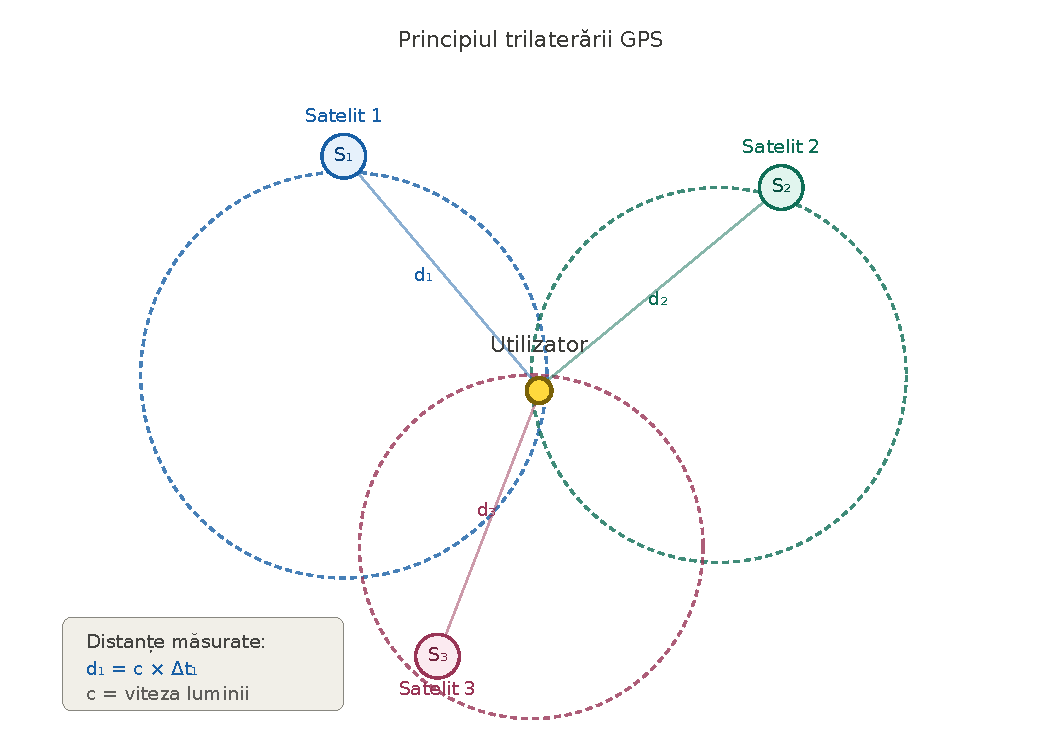
\includegraphics[width=0.75\textwidth]{figuri/trilaterare_gps.pdf}
    \caption{Principiul trilaterării GPS}
    \label{fig:trilaterare}
\end{figure}


Este important de menționat că platforma ETTIway nu implementează principiul de trilaterare.
Procesul matematic de calcul al poziției pe baza semnalelor recepționate de la sateliți este realizat la un nivel mult mai jos, 
în chipset-ul GPS al dispozitivului mobil.

\subsection{Precizia și limitările localizării}
\label{subsec:precizie}

Precizia localizării variază semnificativ în funcție de mediu și de sursele
disponibile. În spațiu deschis, cu vizibilitate directă către sateliți, eroarea
este de ordinul câtorva metri. În schimb, în interiorul clădirilor sau în
apropierea structurilor înalte, semnalul provenit de la sateliți este atenuat ori reflectat.
Precizia este degradată considerabil din aceste cauze, putând ajunge la zeci de metri. Acest
fenomen este deosebit de relevant pentru un campus universitar, unde clădirile
sunt dese și utilizatorii petrec mult timp în interior, exact contextul în care
poziționarea prin semnalele provenite de la sateliți devine cel mai puțin fiabilă.

Din această cauză, un sistem de navigare solid trebuie să trateze explicit
situațiile de imprecizie sau de lipsă temporară a semnalului, evitând afișarea
unei poziții înșelător de exacte și informând utilizatorul cu privire la gradul
de încredere al localizării. În cadrul ETTIway, poziția utilizatorului este
folosită ca un punct de plecare pentru calculul traseului, fiind asociată celui mai
apropiat punct de pe rețeaua de trasee a campusului, astfel încât micile erori de
localizare să nu împiedice funcționarea rutării.

\section{Algoritmi de determinare a drumului minim}
\label{sec:algoritmi-rutare}

Componenta de rutare reprezintă nucleul funcțional al oricărui sistem de
navigare. Odată ce infrastructura campusului este reprezentată sub forma unui
graf, problema găsirii celui mai scurt traseu între două puncte devine o
problemă clasică de teoria grafurilor, ce constă în determinarea drumului de cost minim între
două noduri. Această secțiune prezintă fundamentele teoretice ale problemei și
algoritmii care o rezolvă. Vom pune accent pe soluția folosită în implementare.

\subsection{Modelarea problemei prin grafuri}
\label{subsec:graf-teoretic}

Un graf este o structură formată dintr-un set de noduri și un set de muchii care
leagă perechi de noduri între ele. În contextul navigării, nodurile corespund punctelor de
decizie, intersecții, intrări, capete de alei, iar muchiile corespund
segmentelor de traseu care le unesc, fiecărei muchii i se asociază o pondere,
care exprimă costul parcurgerii segmentului respectiv. În cazul cel mai simplu,
ponderea reprezintă distanța geografică reală dintre cele două noduri, dar pot fi
folosite și alte criterii, precum timpul estimat de parcurgere sau gradul de
accesibilitate.

Atunci când ponderile reprezintă distanțe, graful este nedirecționat, deoarece o
alee poate fi parcursă în ambele sensuri cu același cost. Problema centrală
devine astfel găsirea, în acest graf ponderat, a lanțului de muchii care leagă
nodul de start de nodul de destinație și a cărui sumă a ponderilor este minimă.
Această formulare permite aplicarea unor algoritmi cunoscuți, cum ar fi algoritmul
Dijkstra\cite{Madkour2017}. 

\subsection{Algoritmul Dijkstra}
\label{subsec:dijkstra-teoretic}

Cel mai cunoscut algoritm pentru determinarea drumului minim de la un nod sursă
către celelalte noduri ale unui graf cu ponderi pozitive este algoritmul
Dijkstra. Principiul său de funcționare este unul de tip lacom (\textit{greedy}).
Algoritmul menține, pentru fiecare nod, cea mai mică distanță cunoscută până la
acel moment față de nodul sursă, precum și nodul precedent pe traseul optim. La
fiecare pas, este selectat nodul nevizitat cu distanța minimă, după care se
încearcă îmbunătățirea distanțelor către vecinii săi, operație cunoscută sub
numele de relaxare a muchiilor. Procesul continuă până când nodul de destinație
este atins sau până când toate nodurile accesibile au fost vizitate.

Corectitudinea algoritmului se bazează pe observația că, atunci când un nod este
selectat ca având distanța minimă dintre cele nevizitate, această distanță este
deja optimă și nu mai poate fi îmbunătățită ulterior, întrucât toate ponderile
sunt pozitive. La final, traseul optim se reconstruiește pornind de la nodul de
destinație și urmărind, în sens invers, lanțul nodurilor precedente până la
sursă. Acest mod de funcționare îl face potrivit pentru calculul traseelor într-o
rețea de dimensiuni moderate, cum este cea a unui campus universitar\cite{Columbia_Dijkstra}.

Pentru a ilustra modul de funcționare a algoritmului, Figura~\ref{fig:dijkstra} prezintă un graf cu șase noduri (A până la F) și un set de muchii cu costuri asociate. Algoritmul lui Dijkstra explorează sistematic toate căile posibile de la nodul de plecare și identifică drumul de cost minim către fiecare nod destinație. Pentru exemplul ilustrat, drumul de la A la F cu cost minim este A → B → D → F, cu un cost total de 9 unități, în detrimentul alternativei A → C → E → F, care are un cost total de 15 unități.

\begin{figure}[htbp]
    \centering
    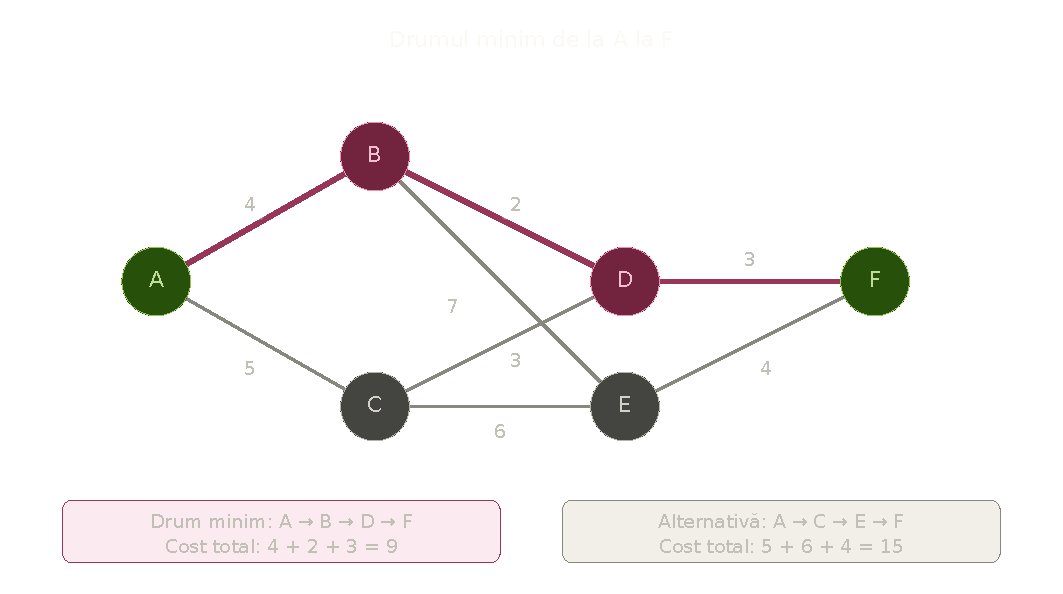
\includegraphics[width=0.85\textwidth]{figuri/dijkstra_exemplu.pdf}
    \caption{Exemplu de aplicare a algoritmului lui Dijkstra.}
    \label{fig:dijkstra}
\end{figure}



\subsection{Performanță și optimizări}
\label{subsec:performanta-rutare}

Performanța algoritmului Dijkstra depinde în mod esențial de modul în care
este implementată operația de selectare a nodului cu distanța minimă. Într-o
implementare directă, în care la fiecare pas se parcurg toate nodurile pentru a-l
găsi pe cel cu distanța minimă, complexitatea devine pătratică în raport cu
numărul de noduri. Pentru grafuri mari, această abordare devine ineficientă, iar
literatura de specialitate propune optimizări bazate pe structuri de date de tip
coadă de priorități, care reduc semnificativ timpul de execuție prin extragerea
rapidă a nodului minim \cite{Chen2022}.

Pentru rețeaua unui campus universitar, în care numărul de noduri este relativ
redus, implementarea directă a algoritmului oferă timpi de răspuns acceptabili,
calculul traseului fiind perceput instantaneu de către utilizator. Tocmai
din acest motiv, în cadrul ETTIway s-a optat pentru o implementare clară și ușor
de urmărit a algoritmului. S-a pus accent pe prioritizarea lizibilității codului în detrimentul unor
optimizări care nu ar fi adus beneficii practice la această scară. Aceleași
principii stau la baza serviciilor de rutare la scară largă construite peste date
deschise precum cele din OpenStreetMap \cite{Luxen2011}, care însă necesită
structuri de date și optimizări mult mai complexe pentru a trata rețele de
dimensiunea unor orașe întregi.




\section{Interfețe pentru dispozitive mobile}
\label{sec:mobil}

Un sistem de navigare în campus este utilizat, natural, preponderent de pe
dispozitive mobile, utilizatorul având nevoie de orientare tocmai atunci când se
deplasează prin campus, telefonul fiind dispozitivul aflat permanent la îndemână.
Din acest motiv, proiectarea interfeței trebuie să țină cont, încă de la început,
de constrângerile specifice ecranelor de mici dimensiuni și ale interacțiunii
tactile.

Principiul de proiectare adecvat acestui context este cel al designului intuitiv.
Interfața se adaptează automat la dimensiunea ecranului pe care este
afișată, reorganizând elementele pentru a rămâne lizibile și utilizabile atât pe
un monitor de calculator, cât și pe ecranul unui telefon. În cazul unei aplicații
de hărți, acest lucru presupune ca harta să ocupe cât mai mult din suprafața
disponibilă, iar elementele de control (căutarea, lista de clădiri, detaliile)
să fie organizate astfel încât să nu obtureze harta, putând fi afișate sau
ascunse după nevoie.

Pe lângă adaptarea vizuală, interacțiunea tactilă impune constrângeri proprii cum ar fi:
elementele care pot fi atinse trebuie să fie suficient de mari pentru a fi
acționate cu degetul, iar gesturile uzuale, deplasarea hărții prin glisare,
mărirea prin apropierea degetelor, trebuie să funcționeze natural. Biblioteca, Leaflet,
folosită pentru afișarea hărții în ETTIway oferă suport nativ pentru aceste
gesturi, ceea ce simplifică obținerea unei experiențe fluide pe dispozitivele
mobile\cite{Leaflet}.


\section{Arhitecturi de aplicații web}
\label{sec:arhitecturi-web}

Platforma ETTIway este construită pe o arhitectură de tip client-server, în care
responsabilitățile sunt separate clar între componenta care rulează în browserul
utilizatorului și componenta care rulează pe server. Această separare este o
practică des întâlnită în dezvoltarea aplicațiilor web moderne.

\subsection{Separarea frontend-backend}
\label{subsec:frontend-backend}

Frontend-ul, adică partea aplicației care rulează în browserul utilizatorului,
este responsabil de prezentarea informației și de interacțiunea directă cu
utilizatorul: afișarea hărții, gestionarea evenimentelor de tip clic, încărcarea
planurilor de etaj și prezentarea detaliilor despre clădiri. Backend-ul, adică
partea care rulează pe server, este responsabil de gestionarea datelor, de
expunerea serviciilor prin care frontend-ul obține informația și de aplicarea
logicii de prelucrare necesare.

Această separare a responsabilităților permite dezvoltarea și testarea
independentă a celor două componente. Frontend-ul poate fi modificat fără a
afecta logica de date, iar backend-ul poate fi extins prin adaugarea unor noi servicii fără a
necesita rescrierea interfeței. Comunicarea dintre cele două straturi se
realizează printr-o interfață bine definită de servicii, ceea ce reduce
cuplarea dintre componente și facilitează evoluția independentă a acestora.

\subsection{Servicii REST și formatul JSON}
\label{subsec:rest-json}

Comunicarea dintre frontend și backend în ETTIway se realizează prin servicii de
tip REST (\textit{Representational State Transfer}). Acest stil arhitectural se
bazează pe protocolul HTTP și organizează accesul la date în jurul noțiunii de
resurse. Fiecare resursă este identificată printr-o adresă și manipulată prin
operațiile standard ale protocolului. Avantajul acestui model constă în
simplitatea pe care o aduce. Un serviciu REST poate fi
consumat de orice client capabil să efectueze cereri HTTP, indiferent de
tehnologia pe care este construit.

Pentru schimbul efectiv de date se folosește formatul JSON (\textit{JavaScript
Object Notation}), un format text ușor de citit atât de oameni, cât și de
mașini, care permite reprezentarea structurată a obiectelor și a colecțiilor.
JSON s-a impus ca format standard în comunicarea dintre aplicațiile web datorită
simplității sale și a suportului nativ existent în limbajul JavaScript, folosit
pentru dezvoltarea frontend-ului \cite{JSONorg}. În cadrul aplicației, datele despre clădiri,
etaje și puncte de interes sunt transmise între server și client sub formă de
obiecte JSON.

\subsection{Rețele private virtuale și topologii de tip mesh}
\label{subsec:mesh}
 
Aplicațiile web care lucrează cu date sensibile sau care sunt destinate unor
comunități restrânse pot beneficia de o expunere controlată, alternativă
expunerii pe internetul public. O astfel de soluție este utilizarea unei rețele
private virtuale (VPN, \textit{Virtual Private Network}), care creează un canal
criptat între dispozitivele autorizate, izolat de traficul public \cite{NIST_VPN}. În cadrul
ETTIway, o asemenea abordare se potrivește atât cu natura limitată a publicului
țintă (comunitatea academică a universității), cât și cu cerința de a evita
configurări complexe de firewall sau de redirecționare de porturi pe routerul
de internet.
 
Există două topologii principale pentru rețele private virtuale, care diferă
prin modul în care traficul circulă între dispozitive. În topologia clasică, de
tip \textbf{hub-and-spoke} (stea), tot traficul trece printr-un server central,
care actionează ca punct de tranzit între toate dispozitivele conectate. Această
arhitectură este simplă din punct de vedere conceptual, dar prezintă
limitări: serverul central este atât un punct unic de eșec, cât si un dezavantaj pentru lățimea de bandă, deoarece tot traficul trebuie să treacă prin el.
 
Topologia alternativă, de tip \textbf{mesh peer-to-peer}, înlocuiește serverul
central printr-o rețea în care fiecare dispozitiv poate comunica direct cu
oricare altul, fără puncte intermediare obligatorii. În această arhitectură,
serverul de coordonare are doar rolul de a anunța dispozitivele unul față de
celălalt și de a facilita stabilirea conexiunilor directe, după care nu mai
intervine în traficul efectiv. Acest model 
oferă latențe mai mici, deoarece datele circulă pe drumul cel mai scurt posibil
între cele două capete.\cite{Tailscale}
 
Implementarea practică a rețelelor de tip mesh se bazează pe protocoale
criptografice moderne, dintre care cel mai răspândit în prezent este
\textbf{WireGuard} \cite{Donenfeld2017}. Acesta este un protocol VPN deschis, conceput cu obiectivul
de a oferi performanță ridicată, simplitate de configurare și o suprafață de
atac redusă comparativ cu protocoale mai vechi. Cheia identității unui
dispozitiv în WireGuard este o pereche de chei criptografice (publică și
privată), iar autentificarea se face exclusiv pe baza acestei chei, fără
necesitatea unor parole sau certificate centralizate. Deoarece 
implementarea este compactă (câteva mii de linii de cod, comparativ cu sute de mii pentru
soluții mai vechi) facilitează auditul de securitate și reduce probabilitatea
unor vulnerabilități.
 
O provocare importantă pentru rețelele peer-to-peer este \textbf{traversarea
NAT-urilor} (\textit{Network Address Translation}), procesul prin care
dispozitivele aflate în spatele unor routere domestice sau corporative pot
stabili conexiuni directe între ele, în pofida faptului că nu au adrese IP
publice. Soluțiile moderne folosesc tehnici precum \textit{STUN} (descoperirea
adresei externe)\cite{RFC8489} și \textit{hole punching} (deschiderea simultană a unor porturi
de către ambele capete), iar în cazurile în care traversarea directă nu este
posibilă, traficul este redirecționat printr-un server intermediar (relay).
Astfel de servere de tranzit sunt folosite ca o soluție de rezervă, traficul
rămânând criptat capăt-la-capăt, fără ca operatorul relay-ului să poată descifra
conținutul.
 
Această arhitectură de tip mesh, bazată pe WireGuard și pe servicii de
coordonare moderne, oferă o alternativă elegantă la expunerea publică a
serviciilor. În ETTIway, ea permite ca serverul aplicației să fie accesibil
exclusiv dispozitivelor invitate explicit, fără adresă IP publică și fără
configurări manuale ale certificatului HTTPS, aspecte detaliate în capitolul de
implementare.

\section{Tehnologii utilizate în implementare}
\label{sec:tehnologii}

În această secțiune sunt prezentate tehnologiile concrete pe care se sprijină
implementarea platformei ETTIway. Alegerea acestor tehnologii a fost ghidată de
mai multe criterii: stabilitatea soluțiilor, disponibilitatea
unei documentații cuprinzătoare, caracterul open-source al instrumentelor și
potrivirea cu cerințele specifice ale unui sistem de navigare în campus.

\subsection{Spring Boot pentru backend}
\label{subsec:spring-boot}

Backend-ul aplicației este realizat cu Spring Boot, un cadru de lucru
(\textit{framework}) pentru limbajul Java, destinat dezvoltării rapide de
aplicații și servicii web. Spring Boot reduce semnificativ efortul de
configurare necesar pornirii unui proiect, oferind un set de convenții și de
componente preconfigurate care permit dezvoltatorului să se concentreze asupra
logicii aplicației, nu asupra detaliilor de infrastructură. Printre avantajele
sale se numără un server web încorporat, un sistem solid de gestiune a
dependențelor și o integrare facilă cu bazele de date.\cite{SpringBoot}



În cadrul ETTIway, Spring Boot este folosit pentru a expune serviciile REST prin
care frontend-ul obține datele despre clădiri și despre infrastructura
campusului, precum și pentru a gestiona accesul la stratul de date. Pentru
interacțiunea cu baza de date se utilizează mecanisme de persistență de tip JPA
(\textit{Java Persistence API}), care permit maparea obiectelor din aplicație pe
înregistrările din baza de date, reducând cantitatea de cod necesar pentru
operațiile uzuale de acces la date.

\subsection{Leaflet și JavaScript pentru frontend}
\label{subsec:leaflet}

Interfața de vizualizare a hărții este construită folosind biblioteca Leaflet, o
bibliotecă JavaScript open-source, dedicată afișării hărților interactive în
browser. Leaflet a fost aleasă \cite{Crickard2014} datorită dimensiunii sale reduse, a performanței
bune și a simplității interfeței de programare. Biblioteca oferă suport nativ
pentru afișarea hărților bazate pe dale, pentru gestionarea nivelurilor de zoom,
pentru adăugarea de markere și pentru organizarea informației pe straturi
distincte care pot fi afișate sau ascunse independent.

Restul logicii de pe partea de client este realizat în JavaScript, fără a apela
la un cadru de lucru complex pentru interfață. Această alegere a fost motivată de
dorința de a păstra aplicația ușoară și de a reduce dependențele externe, în
acord cu obiectivul de a obține timpi de răspuns reduși și o experiență
fluidă. Interfața este structurată într-un panou lateral, care găzduiește
funcțiile de căutare, lista clădirilor disponibile și detaliile clădirii
selectate, și o zonă principală ocupată de harta interactivă. Vizualizarea
planurilor de etaj se realizează printr-o fereastră modală, care permite
parcurgerea nivelurilor unei clădiri fără a părăsi contextul hărții.

\subsection{Organizarea datelor și extensibilitatea}
\label{subsec:organizare-date}

Datele despre clădiri și despre structura lor interioară sunt organizate
într-o formă structurată, care asociază fiecărei clădiri un identificator,
denumirea, poziția geografică, o descriere și lista nivelurilor sale, fiecare
nivel având asociat un plan corespunzător. Această organizare a fost gândită
pentru a fi ușor de extins: adăugarea unei noi clădiri sau a unui nou etaj
presupune completarea structurii de date, fără a fi necesare modificări în
logica aplicației. Extensibilitatea reprezintă un obiectiv explicit al
proiectului, deoarece un campus universitar este un mediu dinamic, în care
infrastructura se modifică în timp, iar o soluție viabilă trebuie să poată
absorbi aceste schimbări cu efort minim.

\section{Concluziile capitolului}
\label{sec:concluzii-cap1}

În acest capitol au fost prezentate fundamentele teoretice și tehnologice care
stau la baza platformei ETTIway. Au fost introduse conceptele de sistem de
navigare digitală și de hartă interactivă, distincția dintre navigarea
exterioară și cea interioară, precum și provocarea integrării acestora într-un
flux unitar. S-au discutat apoi conceptele esențiale legate de datele
geospațiale, sisteme de referință, reprezentarea geometriilor și sursele de
date open-source. A fost analizat mecanismul de poziționare a utilizatorului prin
sistemul GPS, împreună cu limitările sale de precizie în mediul construit. Am atins si subiectul algoritmilor de determinare a drumului minim, cu
accent pe algoritmul Dijkstra, folosit pentru calculul traseelor. În final,
au fost discutate cerințele de proiectare a interfețelor pentru dispozitive
mobile și tehnologiile concrete utilizate în implementare. De la cadrul Spring
Boot pentru backend până la biblioteca Leaflet pentru vizualizarea hărții,
subliniind în fiecare caz motivele care au stat la baza alegerii lor.

Înțelegerea acestor elemente este necesară pentru parcurgerea capitolelor
următoare, în care vor fi prezentate analiza cerințelor, arhitectura detaliată a
sistemului și modul concret de implementare a funcționalităților platformei.
Plecând de la fundamentele expuse aici, următorul capitol abordează cerințele
funcționale și nefuncționale ale aplicației, precum și deciziile de proiectare
care decurg din acestea.
